%------------------------------------------------------------------------------
% Template file for the submission of papers to IUCr journals in LaTeX2e
% using the iucr document class
% Copyright 1999-2013 International Union of Crystallography
% Version 1.6 (28 March 2013)
%------------------------------------------------------------------------------

\documentclass[pdf]{iucr}              % DO NOT DELETE THIS LINE
\RequirePackage{graphicx}
\RequirePackage{url}
\voffset=-0.5in
\RequirePackage{siunitx}

     %-------------------------------------------------------------------------
     % Information about journal to which submitted
     %-------------------------------------------------------------------------
     \journalcode{J}              % Indicate the journal to which submitted
                                  %   A - Acta Crystallographica Section A
                                  %   B - Acta Crystallographica Section B
                                  %   C - Acta Crystallographica Section C
                                  %   D - Acta Crystallographica Section D
                                  %   E - Acta Crystallographica Section E
                                  %   F - Acta Crystallographica Section F
                                  %   J - Journal of Applied Crystallography
                                  %   M - IUCrJ
                                  %   S - Journal of Synchrotron Radiation

\begin{document}                  % DO NOT DELETE THIS LINE

     %-------------------------------------------------------------------------
     % The introductory (header) part of the paper
     %-------------------------------------------------------------------------

     % The title of the paper. Use \shorttitle to indicate an abbreviated title
     % for use in running heads (you will need to uncomment it).

\title{Introducing classical molecular dynamics simulation to users of
scattering}
\shorttitle{Simulation and scattering}

     % Authors' names and addresses. Use \cauthor for the main (contact)
     % author.
     % Use \author for all other authors. Use \aff for authors' affiliations.
     % Use lower-case letters in square brackets to link authors to their
     % affiliations; if there is only one affiliation address, remove the [a].

\cauthor[a,b]{Andrew R.}{McCluskey}{a.r.mccluskey@bath.ac.uk}{}
\author[a]{Adam R.}{Symington}
\author[c]{James}{Grant}
\author[a]{Benjamin J.}{Morgan}
\author[a]{Stephen C.}{Parker}
\cauthor[a]{Karen J.}{Edler}{k.edler@bath.ac.uk}

\aff[a]{Department of Chemistry, University of Bath, Claverton Down, Bath,
BA2 7AY \country{UK}}
\aff[b]{Diamond Light Source, Diamond House, Rutherford Appleton Laboratory,
Harwell Oxford, OX11 0DE, \country{UK}}
\aff[c]{Department of Chemistry, University of Bath, Claverton Down, Bath,
BA2 7AY \country{UK}}

     % Use \shortauthor to indicate an abbreviated author list for use in
     % running heads (you will need to uncomment it).

\shortauthor{McCluskey, Symington, Grant, Morgan, Edler, and Parker}

     % Use \vita if required to give biographical details (for authors of
     % invited review papers only). Uncomment it.

%\vita{Author's biography}

     % Keywords (required for Journal of Synchrotron Radiation only)
     % Use the \keyword macro for each word or phrase, e.g.
     % \keyword{X-ray diffraction}\keyword{muscle}

%\keyword{keyword}

     % PDB and NDB reference codes for structures referenced in the article and
     % deposited with the Protein Data Bank and Nucleic Acids Database (Acta
     % Crystallographica Section D). Repeat for each separate structure e.g
     % \PDBref[dethiobiotin synthetase]{1byi} \NDBref[d(G$_4$CGC$_4$)]{ad0002}

%\PDBref[optional name]{refcode}
%\NDBref[optional name]{refcode}

\maketitle                        % DO NOT DELETE THIS LINE

\begin{synopsis}
We describe an open educational resource for the introduction of classical molecular dynamics to the users of scattering techniques.
The purpose of this is to enable scattering domain experts to learn about these simulation techniques.
The better understanding that this will facilitate in the users will allow for better application of these techniques as an aspect of multi-modal analysis for scattering data.
\end{synopsis}

\begin{abstract}
Classical molecular dynamics simulations are becoming a popular technique for the multi-modal analysis of scattering techniques; such as small angle scattering and diffraction.
However, few users of these techniques have formalised training in these methodologies, resulting in frequent use of molecular dynamics simulations as a black box technique.
This work discusses an open educational resource designed to introduce classical molecular dynamics to users of scattering, describing possible sources of error in the method.
Furthermore, we cover some of the methods that can be used to enable simulation techniques to facilitate in the analysis of scattering data.
\end{abstract}


     %-------------------------------------------------------------------------
     % The main body of the paper
     %-------------------------------------------------------------------------
     % Now enter the text of the document in multiple \section's, \subsection's
     % and \subsubsection's as required.

\section{Introduction}

The use of molecular dynamics simulations to aid in the analysis of experimental data; particular from small angle scattering and diffraction, has grown significantly over the past ten years \cite{Pan2012,Boldon2015,Hub2018,Ivanovic2018,East2016,Wall2014,Wall2018,Satoh2015}.
Figure \ref{fig:growth} shows the growth in the percentage of small angle scattering (SAS) publications that mention molecular dynamics.
It can be seen that there has been a linear growth in such publications, with more than \SI{20}{\percent} of all SAS publications mentioning molecular dynamics as of 2018.
This alone is a clear indication of the importance simulation techniques are having on the field of scattering and diffraction.

Normally, the users of scattering and diffraction techniques have a background in experimental science, with little or no formalised training in computational modelling techniques.
This may be problematic, as it can lead to the use of molecular simulation as a black-box, with little understanding or consideration for the underlying methodologies.
The use of molecular simulation in this fashion can quickly lead to the inclusion of severe, systematic errors.
This has lead to the development of tools, such as WAXSiS or SASSIE \cite{Chen2014,Knight2015,Perkins2016}, that present easy-to-use interfaces designed to reduce the risk of these errors.

In addition to the development of software packages, another method to further limit systematic errors, are lectures or courses presenting and introduction to molecular simulation for scattering and diffraction users.
For example, the annual ISIS Neutron Training Course now included an ``Introduction to Molecular Dyanmics for Neutron Scattering'' module.
This details the fundemental of classical molecular dynamics simulation, before presenting some previous applications of these methods in neutron science and allowing the students to gain a familiarity with the SASSIE package.
While such courses and modules are an important aspect of training, they are limited both in numbers of students that may attend and location, meaning that not scattering and diffraction users may easily access them.

There has been a recent movement within the scientific and engineering communities towards technology-enchanced open educational resources (OERs).
These are courses, lectures, or learning modules that are made free available online for use by anyone.
This allows the permission for others to engage in the ``5R activities'': Retain, Reuse, Revise, Remix, and Redistribute \cite{opencontent2018}.
The act of publishing an OER increases the reach of a particular resource as it allows others to pick it up, modify it, and use the modified version in their own teaching.
The availability of the Jupyter Notebook framework \cite{Kluyver2016} has facilitated the availability of OERs by improving the ability for students to interact directly with the resource using, often but not always, the Python programming language \cite{Barba2017}.

Herein, we present an online, open-source, interactive module aimed to introduce members of the scattering and diffraction community to molecular dynamics simulation.
This course follows six lessons, covering classical methods, introducing molecular dynamics, and showing how this method may interact with scattering in a multi-modal fashion.
We leverage the open-source Python library pylj \cite{McCluskey2018} to give a visual, and programmatic representation of the interaction between these two techniques.
In this paper, we will discuss the implementation of the module, and detail how the student (in this work \emph{the student} refers to any student of the module regardless of career position) may get the most from the module.

\section{Assumed prior knowledge}

The OER, entitled \emph{``The interaction between simulation and scattering''} makes use of the Python programming language, this allows for interactive examples of the mathematical and algorithm content to be included.
A result of this is that, to be able to fully utilise the course, some knowledge, of willingness to learn, Python is required.
However, we have attempted to develop the course in such a fashion that an in depth knowledge of Python is not required.
It is anticipated that the users of this course would have some familiarity with undergraduate chemistry or physics, and the associated level of mathematics.
This is particularly important when considering the nature, and chemical rationale, of the classical interaction potentials.

\section{Module construction}

The module is currently available online, at \url{https://arm61.github.io/sim_and_scat}.
These webpages were written as a series of Jupyter Notebooks and compiled using the build-system developed within the University of Bath.
The use of this system allows for Python code blocks to be easily build into the lessons to give algorihtmic details and facilitate interactivity.
It is expected that the student would use the online material alongside a locally running Jupyter Notebook (the installation of which is detail in the module introduction).
Interacting with the module in this fashion will allow the student to copy the Python code from the web interface, run it locally, and alter the code as they see fit.

The module is provided under a CC-BY-SA-4.0 license, and builds on the growing library of open educational resources.
The open-source nature of this license means that anyone may use the material to enhance their own educational platform, and experts in the field may contribute to improve the module.
The source code for the module is available at \url{https://github.com/arm61/sim_and_scat}.

\section{Module outline}

The module follows a simple outline, with code blocks that gradually build up the students understanding of the concepts.

\subsection{Getting started}

The first page, nominally Lesson 0, introduces the course and outlines the content.
It also gives directions on how to install the necessary software, namely Anaconda Python, and the pylj package \cite{McCluskey2018}, and launch the Jupyter Notebook interface \cite{Kluyver2016}.
It is important that this is introduced early in the module such that students can immediately be actively involves in the interactive experience of the lessons.

\subsection{Classical methods}

Once the students computer is able to run the necessary software, concepts of classical simulation methods are introduced.
These include the nature of potential models and show some examples such as the Lennard-Jones and Buckingham potentials \cite{LennardJones1924,Buckingham1938}.
The course gives a brief description of how a potential model is determined, including mention to the parameterisation from higher accuracy quantum mechanical calculations.
The existence of off-the-shelf potential models is mentioned alongside a discussion of the problems associated with these as they also may require system specific optimisation.
Finally, we mention mixing rules for off-the-shelf potential models, and again discuss possible problems that a user may encounter related to system specificity.

\subsection{Molecular dynamics}

Once the basics of classical methods have been introduced, the student is presented with molecular dynamics.
This is shown by gradually building up a one-dimension molecular dynamics simulation using the Velocity-Verlet algorithm \cite{Swope1982} and the Lennard-Jones potential model \cite{LennardJones1924}.
This begins by detailing the requirement to find the forces on the particles, before introducing how the acceleration is determined for each particle.
Finally, the different aspects of the determination of the particle positions and velocities using the Velocity-Verlet algorithm are outlined.

\subsection{pylj and the interaction with scattering}

The final aspect of the module makes use of the Python package pylj \cite{McCluskey2018}.
This is a open-source package designed to introduce students to classical atomistic simulation.
First, the student is given a working pylj molecular dynamics simulation to run on locally, then they are shown how to use the custom plot functionality of pylj to present information about the simulation.
In the final lesson, the Debye equation is introduced and the students are shown how to implement it within pylj.
Using pylj, the students may then observe the effect of temperature on both the structure of the argon particles, in addition to the scattering profile that is generated from the Debye equation.
Finally, we mention the algorithms that may be used to improve the efficiency of the calculation of the scattering profile, such as the Fibonacci sequence or the Golden Vectors method \cite{Svergun1994, Watson2013}.

\section{Future outlook}

In future, we hope that the open-source nature of the module will allow interested parties to use and build upon it.
Furthermore, we welcome student input to improve implementation and pedagogical aspects of the module.
We hope to use this module within teaching at courses such as the ISIS Neutron Training Course and the Diamond SAS workshop, from which feedback may be obtained directly.


     % Appendices appear after the main body of the text. They are prefixed by
     % a single \appendix declaration, and are then structured just like the
     % body text.

%\appendix
%\section{Appendix title}

%Text text text text text text text text text text text text text text
%text text text text text text text.

%\subsection{Title}

%Text text text text text text text text text text text text text text
%text text text text text text text.

%\subsubsection{Title}

%Text text text text text text text text text text text text text text
%text text text text text text text.


     %-------------------------------------------------------------------------
     % The back matter of the paper - acknowledgements and references
     %-------------------------------------------------------------------------

     % Acknowledgements come after the appendices

\ack{A. R. M. is grateful to the University of Bath and Diamond Light Source for co-funding a studentship (Studentship Number STU0149).
B. J. M. acknowledges support from the Royal Society (Grant No. UF130329).}

     % References are at the end of the document, between \begin{references}
     % and \end{references} tags. Each reference is in a \reference entry.

%\begin{references}
\bibliographystyle{iucr}
\bibliography{iucr.bib}
%\end{references}

     %-------------------------------------------------------------------------
     % TABLES AND FIGURES SHOULD BE INSERTED AFTER THE MAIN BODY OF THE TEXT
     %-------------------------------------------------------------------------

     % Simple tables should use the tabular environment according to this
     % model

%\begin{table}
%\caption{Caption to table}
%\begin{tabular}{llcr}      % Alignment for each cell: l=left, c=center, r=right
% HEADING    & FOR        & EACH       & COLUMN     \\
%\hline
% entry      & entry      & entry      & entry      \\
% entry      & entry      & entry      & entry      \\
% entry      & entry      & entry      & entry      \\
%\end{tabular}
%\end{table}
%
\begin{figure}
\caption{The annual growth of the percentage of publication that mention ``small angle scattering'' which also mention ``molecular dynamics. Determined from the number of results from a Google Scholar search.}
\label{fig:growth}
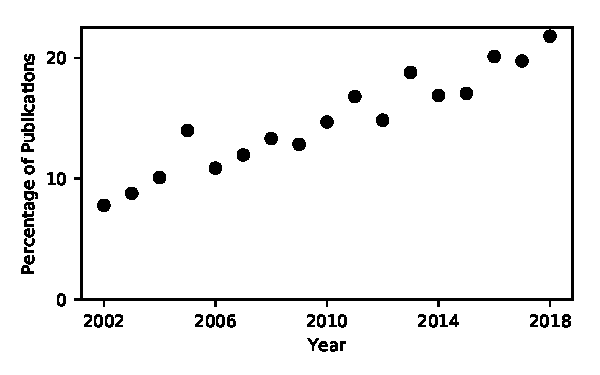
\includegraphics[width=\textwidth]{figures/chem_data_py.pdf}
\end{figure}
%


\end{document}                    % DO NOT DELETE THIS LINE
%%%%%%%%%%%%%%%%%%%%%%%%%%%%%%%%%%%%%%%%%%%%%%%%%%%%%%%%%%%%%%%%%%%%%%%%%%%%%%
